% Options for packages loaded elsewhere
\PassOptionsToPackage{unicode}{hyperref}
\PassOptionsToPackage{hyphens}{url}
\PassOptionsToPackage{dvipsnames,svgnames,x11names}{xcolor}
%
\documentclass[
  ignorenonframetext,
]{beamer}
\usepackage{pgfpages}
\setbeamertemplate{caption}[numbered]
\setbeamertemplate{caption label separator}{: }
\setbeamercolor{caption name}{fg=normal text.fg}
\beamertemplatenavigationsymbolsempty
% Prevent slide breaks in the middle of a paragraph
\widowpenalties 1 10000
\raggedbottom
\setbeamertemplate{part page}{
  \centering
  \begin{beamercolorbox}[sep=16pt,center]{part title}
    \usebeamerfont{part title}\insertpart\par
  \end{beamercolorbox}
}
\setbeamertemplate{section page}{
  \centering
  \begin{beamercolorbox}[sep=12pt,center]{part title}
    \usebeamerfont{section title}\insertsection\par
  \end{beamercolorbox}
}
\setbeamertemplate{subsection page}{
  \centering
  \begin{beamercolorbox}[sep=8pt,center]{part title}
    \usebeamerfont{subsection title}\insertsubsection\par
  \end{beamercolorbox}
}
\AtBeginPart{
  \frame{\partpage}
}
\AtBeginSection{
  \ifbibliography
  \else
    \frame{\sectionpage}
  \fi
}
\AtBeginSubsection{
  \frame{\subsectionpage}
}
\usepackage{amsmath,amssymb}
\usepackage{lmodern}
\usepackage{iftex}
\ifPDFTeX
  \usepackage[T1]{fontenc}
  \usepackage[utf8]{inputenc}
  \usepackage{textcomp} % provide euro and other symbols
\else % if luatex or xetex
  \usepackage{unicode-math}
  \defaultfontfeatures{Scale=MatchLowercase}
  \defaultfontfeatures[\rmfamily]{Ligatures=TeX,Scale=1}
\fi
% Use upquote if available, for straight quotes in verbatim environments
\IfFileExists{upquote.sty}{\usepackage{upquote}}{}
\IfFileExists{microtype.sty}{% use microtype if available
  \usepackage[]{microtype}
  \UseMicrotypeSet[protrusion]{basicmath} % disable protrusion for tt fonts
}{}
\makeatletter
\@ifundefined{KOMAClassName}{% if non-KOMA class
  \IfFileExists{parskip.sty}{%
    \usepackage{parskip}
  }{% else
    \setlength{\parindent}{0pt}
    \setlength{\parskip}{6pt plus 2pt minus 1pt}}
}{% if KOMA class
  \KOMAoptions{parskip=half}}
\makeatother
\usepackage{xcolor}
\IfFileExists{xurl.sty}{\usepackage{xurl}}{} % add URL line breaks if available
\IfFileExists{bookmark.sty}{\usepackage{bookmark}}{\usepackage{hyperref}}
\hypersetup{
  pdftitle={Bias},
  colorlinks=true,
  linkcolor={blue},
  filecolor={Maroon},
  citecolor={Blue},
  urlcolor={Blue},
  pdfcreator={LaTeX via pandoc}}
\urlstyle{same} % disable monospaced font for URLs
\newif\ifbibliography
\usepackage{longtable,booktabs,array}
\usepackage{calc} % for calculating minipage widths
\usepackage{caption}
% Make caption package work with longtable
\makeatletter
\def\fnum@table{\tablename~\thetable}
\makeatother
\usepackage{graphicx}
\makeatletter
\def\maxwidth{\ifdim\Gin@nat@width>\linewidth\linewidth\else\Gin@nat@width\fi}
\def\maxheight{\ifdim\Gin@nat@height>\textheight\textheight\else\Gin@nat@height\fi}
\makeatother
% Scale images if necessary, so that they will not overflow the page
% margins by default, and it is still possible to overwrite the defaults
% using explicit options in \includegraphics[width, height, ...]{}
\setkeys{Gin}{width=\maxwidth,height=\maxheight,keepaspectratio}
% Set default figure placement to htbp
\makeatletter
\def\fps@figure{htbp}
\makeatother
\setlength{\emergencystretch}{3em} % prevent overfull lines
\providecommand{\tightlist}{%
  \setlength{\itemsep}{0pt}\setlength{\parskip}{0pt}}
\setcounter{secnumdepth}{-\maxdimen} % remove section numbering
\makeatletter
\makeatother
\makeatletter
\@ifpackageloaded{caption}{}{\usepackage{caption}}
\AtBeginDocument{%
\renewcommand*\contentsname{Table of contents}
\renewcommand*\listfigurename{List of Figures}
\renewcommand*\listtablename{List of Tables}
\renewcommand*\figurename{Figure}
\renewcommand*\tablename{Table}
}
\@ifpackageloaded{float}{}{\usepackage{float}}
\floatstyle{ruled}
\@ifundefined{c@chapter}{\newfloat{codelisting}{h}{lop}}{\newfloat{codelisting}{h}{lop}[chapter]}
\floatname{codelisting}{Listing}
\newcommand*\listoflistings{\listof{codelisting}{List of Listings}}
\makeatother
\makeatletter
\@ifpackageloaded{caption}{}{\usepackage{caption}}
\@ifpackageloaded{subcaption}{}{\usepackage{subcaption}}
\makeatother
\makeatletter
\makeatother
\ifLuaTeX
  \usepackage{selnolig}  % disable illegal ligatures
\fi

\title{Bias}
\author{}
\date{}

\begin{document}
\frame{\titlepage}

\begin{frame}{What is Bias?}
\protect\hypertarget{what-is-bias}{}
\begin{itemize}
\item
  first biased estimator we've focused on was using (N - 1) instead of N
  for variance and standard deviation
\item
  three ways that statistical bias can enter the modeling process is
  from

  \begin{itemize}
  \item
    things biasing the parameter estimates
  \item
    things biasing SEs and CIs
  \item
    things biasing test statistics and p-values
  \end{itemize}
\end{itemize}
\end{frame}

\begin{frame}{Outliers}
\protect\hypertarget{outliers}{}
\begin{itemize}
\item
  an \textbf{outlier} is a score very different from the rest of the
  data
\item
  when looking at bias in boxplots on SPSS, it will provide you with
  information on outliers and \emph{influential} outliers
\item
  researchers say that participants outside +-3SD are considered
  outliers
\item
  outliers bias parameter estimates, but they have a greater impact on
  the error associated with teh estimate
\end{itemize}
\end{frame}

\begin{frame}[fragile]{Outliers}
\protect\hypertarget{outliers-1}{}
\begin{columns}[T]
\begin{column}{0.3\textwidth}
\begin{verbatim}
[1] 20.09062
\end{verbatim}

\begin{verbatim}
[1] 6.026948
\end{verbatim}

\begin{verbatim}
[1] 38.17147
\end{verbatim}

\begin{verbatim}
[1] 2.009781
\end{verbatim}
\end{column}

\begin{column}{0.7\textwidth}
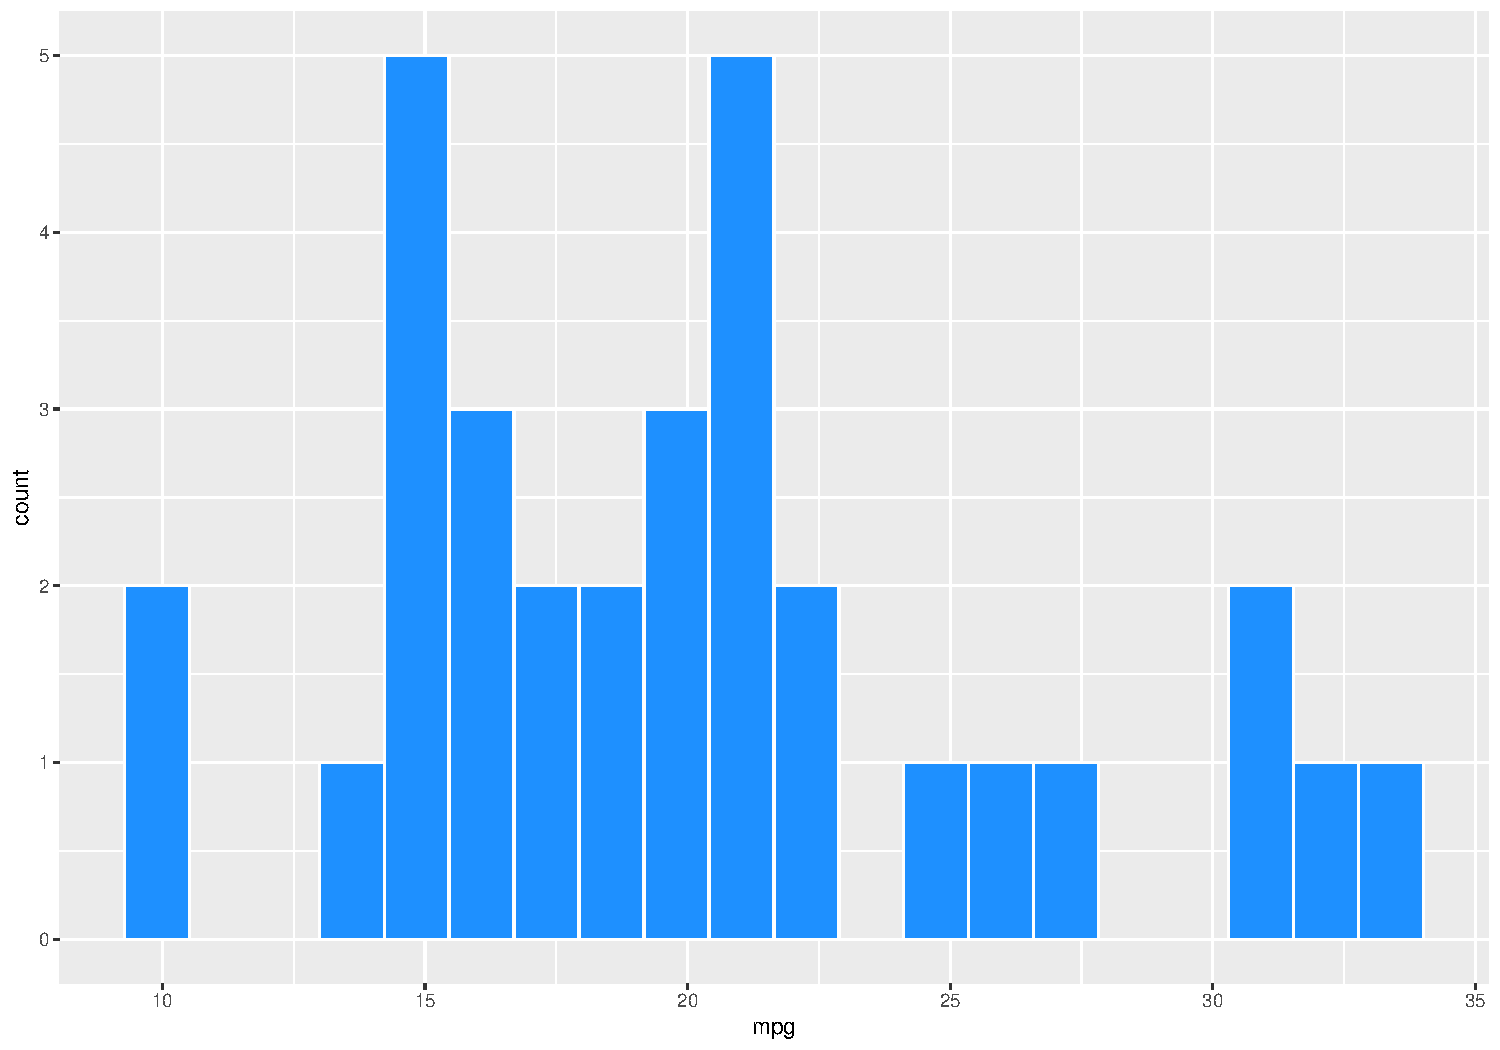
\includegraphics{bias_files/figure-beamer/unnamed-chunk-4-1.pdf}
\end{column}
\end{columns}
\end{frame}

\begin{frame}{Outliers}
\protect\hypertarget{outliers-2}{}
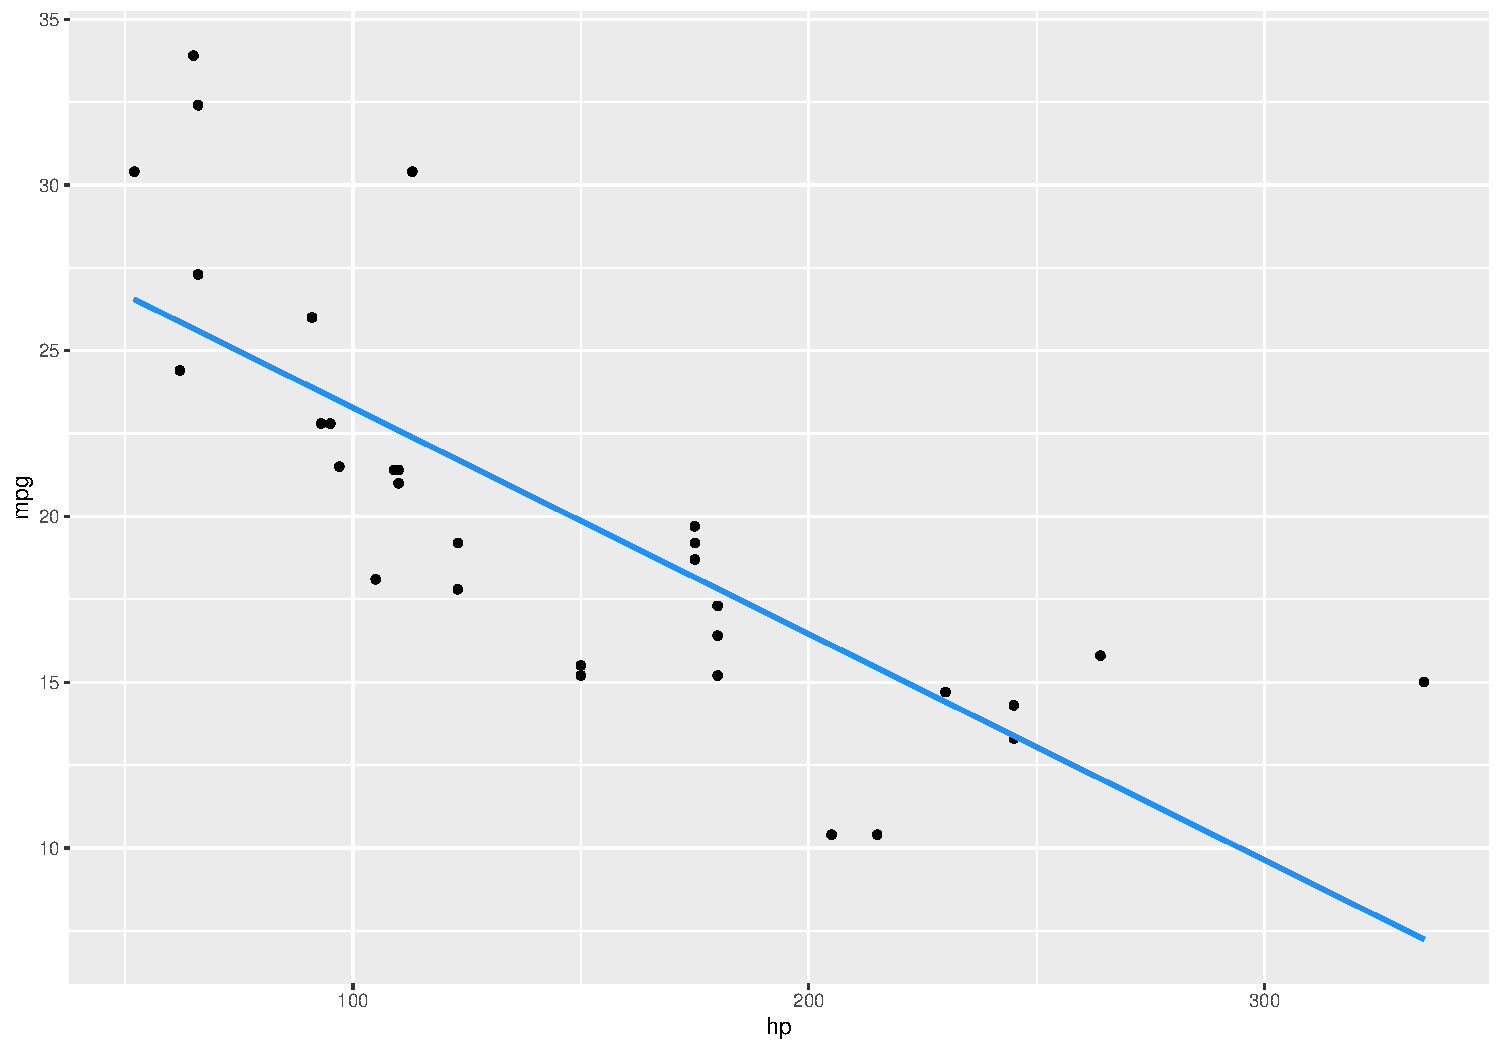
\includegraphics{bias_files/figure-beamer/unnamed-chunk-6-1.pdf}
\end{frame}

\begin{frame}{Assumptions}
\protect\hypertarget{assumptions}{}
\begin{itemize}
\item
  Good researchers will always check the following assumptions before
  conducting inferential statistics

  \begin{itemize}
  \item
    JP: I will warn you right now. \textbf{There are no 100\% correct
    answers to these questions}.

    \begin{itemize}
    \tightlist
    \item
      Statistics is about to get ugly
    \end{itemize}
  \end{itemize}
\item
  If any of the assumptions are violated, your test statistic and
  corresponding p-value may not be correct
\item
  each model you run will have assumptions that need to be checked

  \begin{itemize}
  \tightlist
  \item
    we will talk about these every time we discuss a new test statistic
  \end{itemize}
\item
  The main assumptions are

  \begin{itemize}
  \item
    additivity and linearity
  \item
    normality
  \item
    homoscedasticity/homogeneity of variance
  \item
    independence
  \end{itemize}
\end{itemize}
\end{frame}

\begin{frame}{Additivity \& Linearity}
\protect\hypertarget{additivity-linearity}{}
\begin{itemize}
\item
  many of the models we'll cover are based on linear relationships

  \begin{itemize}
  \tightlist
  \item
    even those that are comparing conditions/groups (e.g., t-tests)
  \end{itemize}
\item
  This assumption is simply based on whether there is a line that fits
  the data \textbf{\emph{well}}

  \begin{itemize}
  \tightlist
  \item
    very subjective
  \end{itemize}
\item
  Every other assumption falls on linearity because if you think you are
  looking at a linear relationship, you want to test it with a linear
  test
\end{itemize}
\end{frame}

\begin{frame}{Additivity \& Linearity}
\protect\hypertarget{additivity-linearity-1}{}
\begin{columns}[T]
\begin{column}{0.5\textwidth}
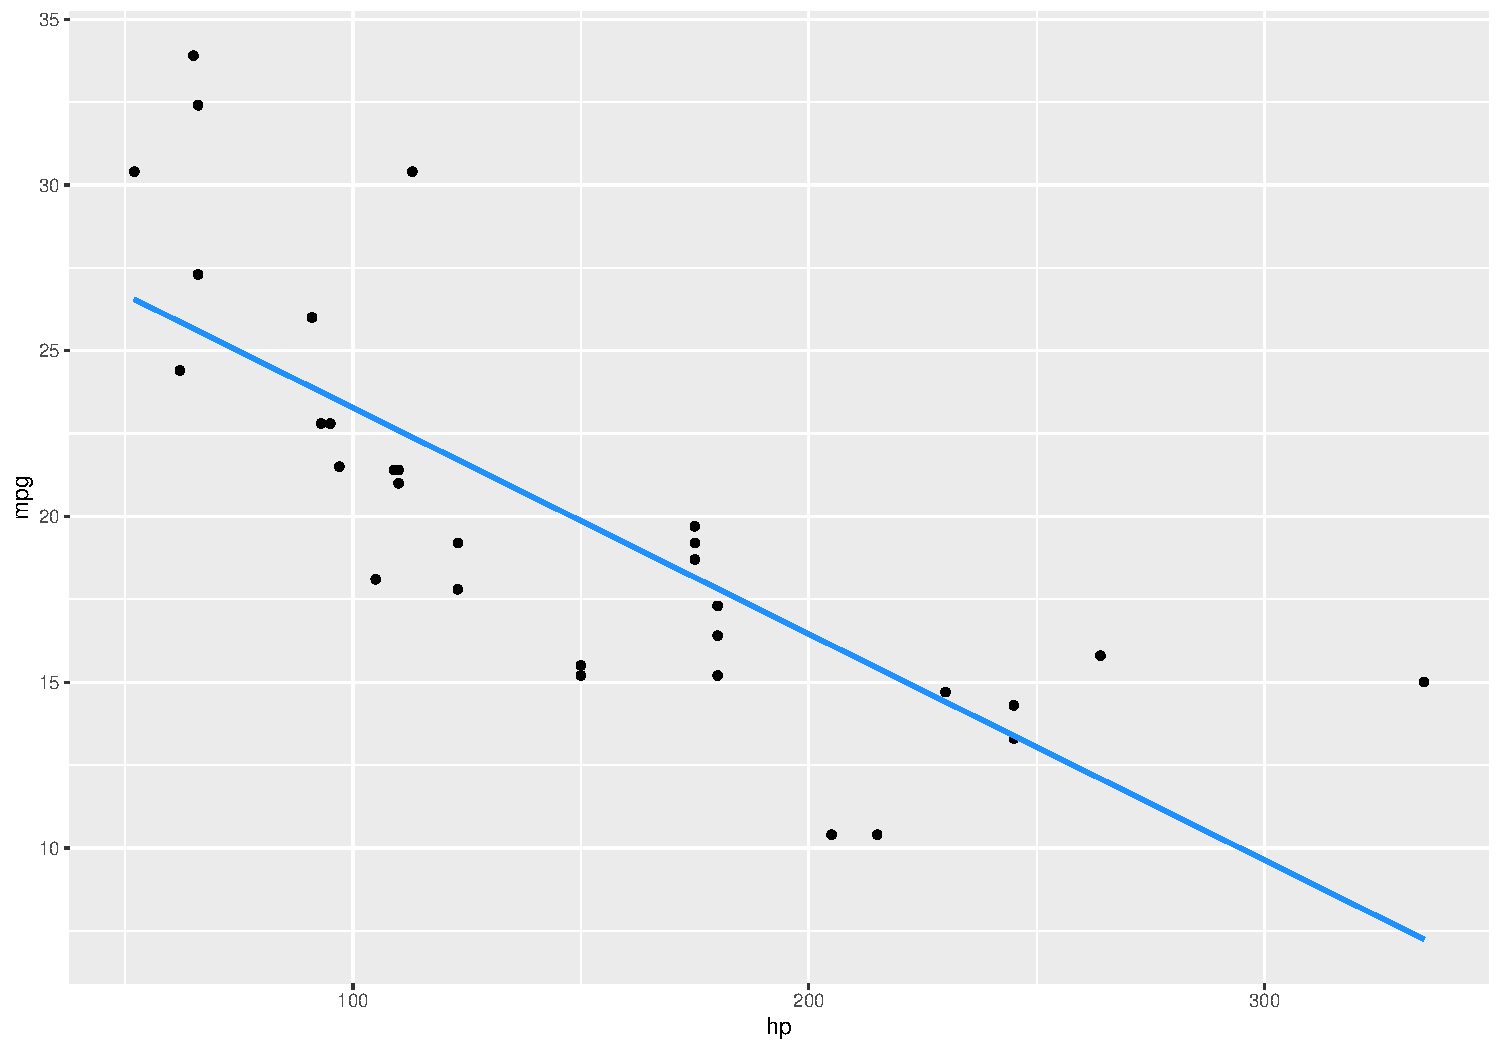
\includegraphics{bias_files/figure-beamer/unnamed-chunk-8-1.pdf}
\end{column}

\begin{column}{0.5\textwidth}
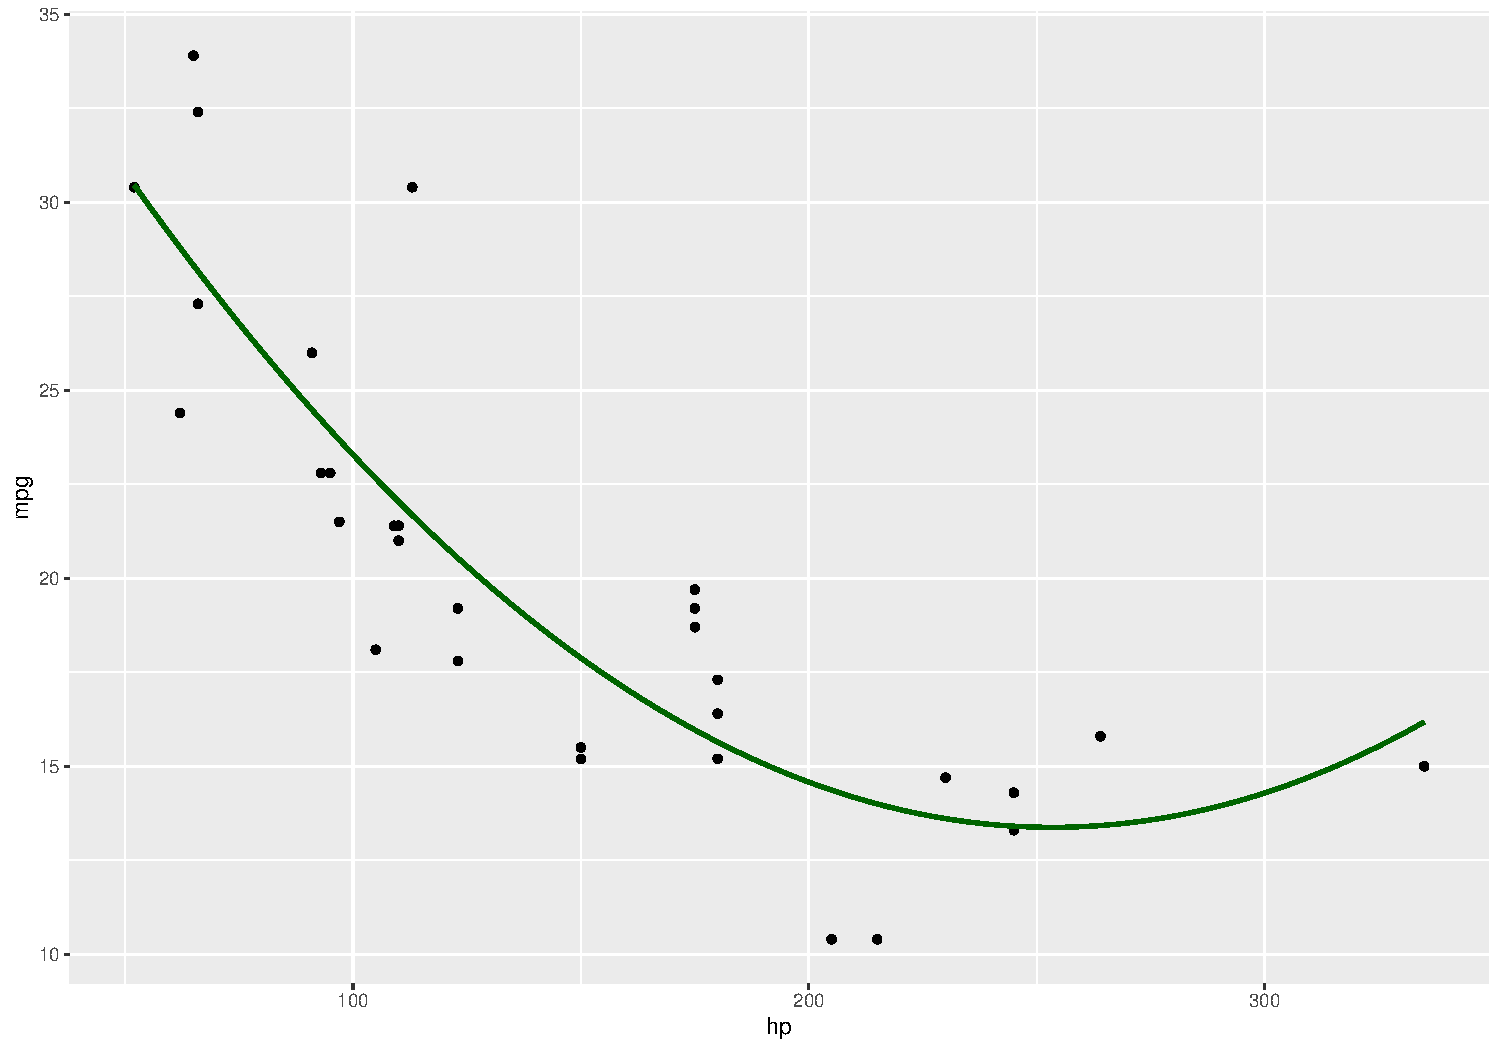
\includegraphics{bias_files/figure-beamer/unnamed-chunk-10-1.pdf}
\end{column}
\end{columns}
\end{frame}

\begin{frame}{Normally Distributed}
\protect\hypertarget{normally-distributed}{}
\begin{itemize}
\item
  many think that your data must be normally distributed

  \begin{itemize}
  \tightlist
  \item
    not the case
  \end{itemize}
\item
  parameter estimates

  \begin{itemize}
  \item
    when we create a model, we have what we predicted in the model and
    the rest (error/deviance/residual)
  \item
    what should be normally distributed are the residuals for the model
  \end{itemize}
\item
  confidence intervals

  \begin{itemize}
  \tightlist
  \item
    for confidence intervals to be accurate, your estimate (what you're
    predicting in your model) should have a normal sampling distribution
  \end{itemize}
\item
  null-hypothesis significance testing

  \begin{itemize}
  \tightlist
  \item
    if your parameter estimates are normal, then the test-statistic
    distribution should also be normally distributed, which would also
    make your alpha/p-value accurate
  \end{itemize}
\end{itemize}
\end{frame}

\begin{frame}{Central Limit Theorem}
\protect\hypertarget{central-limit-theorem}{}
\begin{itemize}
\item
  populations should be normally distributed

  \begin{itemize}
  \tightlist
  \item
    if you have enough observations, your population's distribution will
    be normal
  \end{itemize}
\end{itemize}
\end{frame}

\begin{frame}{Assumption of Normality}
\protect\hypertarget{assumption-of-normality}{}
\begin{itemize}
\item
  confidence intervals don't need to be worried about too much for
  normality because if our parameter estimate is normal then so are our
  confidence intervals if the sample is large enough
\item
  significant tests of models will be accurate if the sample is large
  enough thanks to the central limit theorem
\item
  in estimates of model parameters, residuals of the population must be
  normally distributed
\end{itemize}
\end{frame}

\begin{frame}{Homoscedasticity/Homogeneity of Variance}
\protect\hypertarget{homoscedasticityhomogeneity-of-variance}{}
\begin{itemize}
\item
  homoscedasticity affects parameters and NHST

  \begin{itemize}
  \item
    \textbf{parameters} using Ordinary Least Squares (OLS) estimation,
    we get the best model fit when variance of the DV is equal across
    different values of the IV

    \begin{itemize}
    \tightlist
    \item
      variance is equal across our groups
    \end{itemize}
  \end{itemize}
\item
  \textbf{null hypothesis significance testing} assume variance of the
  outcome if equal across different values of the IV

  \begin{itemize}
  \tightlist
  \item
    some tests (like t-tests) can account for the variance not being
    equal in groups
  \end{itemize}
\end{itemize}
\end{frame}

\begin{frame}{What is Homosceasticity/Homogeneity of Variance?}
\protect\hypertarget{what-is-homosceasticityhomogeneity-of-variance}{}
\begin{itemize}
\item
  \textbf{homoscedasticity} in correlational studies states that
  variance of the DV scores should be stable at all points of the IV

  \begin{itemize}
  \tightlist
  \item
    \textbf{homogeneity of variance} means that all the values should be
    fairly grouped together across each group/all points of the IV
  \end{itemize}
\item
  \textbf{heteroscedasticity} is when the variance of the DV scores is
  different at different points of the IV or different amount groups

  \begin{itemize}
  \tightlist
  \item
    if we were to use error bars (we'll talk about this later), then we
    can see that the points would be spread out more across each group,
    also called \textbf{heterogeneity of variance}
  \end{itemize}
\end{itemize}
\end{frame}

\begin{frame}{When does it matter?}
\protect\hypertarget{when-does-it-matter}{}
\begin{itemize}
\item
  the best fitting model will have homoscedasticity

  \begin{itemize}
  \item
    OLS models will still show model fit, but it won't be the best it
    could be
  \item
    other options can fit the model better like \textbf{weighted least
    squares}, which is when each participant is weighted by a function
    of its variance (adjusts each participant)
  \end{itemize}
\item
  heteroscedasticity can result in biased standard errors, which then
  affects confidence intervals, p values, and parameter estimates
\end{itemize}
\end{frame}

\begin{frame}{Independence}
\protect\hypertarget{independence}{}
\begin{itemize}
\item
  simply put, this means that your errors in your model are not related
  to one another
\item
  JP: I like to work with spatial data, and that tends to have problems
  with independence

  \begin{itemize}
  \tightlist
  \item
    Ex: if I am focusing on different counties, how different are LA
    county and Orange county
  \end{itemize}
\end{itemize}
\end{frame}

\begin{frame}{Spotting Outliers}
\protect\hypertarget{spotting-outliers}{}
\begin{itemize}
\item
  Visuals are the best method to spot outliers easily

  \begin{itemize}
  \item
    histograms
  \item
    boxplots
  \end{itemize}
\item
  boxplots are extremely helpful in SPSS because they show outliers and
  influential outliers
\item
  JP: I tend to run my analyses with both outliers included and dropped
  from the model

  \begin{itemize}
  \tightlist
  \item
    just because they are an extreme case does not mean they are not a
    valid case
  \end{itemize}
\end{itemize}
\end{frame}

\begin{frame}{Spotting Normality}
\protect\hypertarget{spotting-normality}{}
\begin{itemize}
\item
  \textbf{p-p plot} (probability-probability plot) and \textbf{q-q plot}
  (quantile-quantile plot)

  \begin{itemize}
  \item
    p-p plots show the cumulative probability of a variable against the
    cumulative probability of a particular distribution
  \item
    q-q plots show quantiles as dots rather than individual
    points/participants

    \begin{itemize}
    \tightlist
    \item
      essentially, what we want is for our dots to follow the line as
      close as possible for both
    \end{itemize}
  \end{itemize}
\end{itemize}
\end{frame}

\begin{frame}{Using Numbers for Normality}
\protect\hypertarget{using-numbers-for-normality}{}
\begin{itemize}
\item
  we can use measures of central tendency and measures of variability to
  get a better understanding of our data

  \begin{itemize}
  \item
    we can look for minimum and maximum values (outliers)
  \item
    we can see if the SD is large, then there is a lot of
    dispersion/spread/distance between points
  \end{itemize}
\item
  JP: the visuals are just much easier to gather this information from

  \begin{itemize}
  \tightlist
  \item
    afterward, you can check the numbers
  \end{itemize}
\item
  There are also tests to show normality in the data

  \begin{itemize}
  \item
    \textbf{Kolmogorov-Smirnov} and \textbf{Shapiro-Wilk} tests compare
    the scores in a sample to a normally distributed set of scores with
    the same mean and SD
  \item
    if the test is significant, your data is not normal

    \begin{itemize}
    \tightlist
    \item
      not really all that useful because large samples (N
      \textasciitilde{} 150+) can make them be statistically significant
    \end{itemize}
  \end{itemize}
\item
  I'll also cover how to get descriptive statistics for groups

  \begin{itemize}
  \tightlist
  \item
    not entirely relevant because our test statistics will give us that
    information anyway
  \end{itemize}
\end{itemize}
\end{frame}

\begin{frame}{Spotting Linearity}
\protect\hypertarget{spotting-linearity}{}
\begin{itemize}
\item
  in SPSS, spotting problems with linearity and homoscedasticity are
  related to using the residuals

  \begin{itemize}
  \tightlist
  \item
    in SPSS, its sometimes referred to as the \emph{zpred vs zresid.} if
    you transform your variables into z-scores
  \end{itemize}
\item
  JP: I like to look at the raw values in a scatterplot as well as the
  residuals
\item
  points should always look like no general pattern is forming

  \begin{itemize}
  \item
    funnel/fanning= BAD
  \item
    non-linear pattern = BAD
  \item
    fanning \& non linear = BAD
  \end{itemize}
\end{itemize}
\end{frame}

\begin{frame}{Spotting Heteroscedasticity}
\protect\hypertarget{spotting-heteroscedasticity}{}
\begin{itemize}
\item
  \textbf{Levene's test} is a specific test to address whether the
  variance in your groups (categorical IVs) is equal (similar enough) to
  one another

  \begin{itemize}
  \tightlist
  \item
    Ex: Are hours of sleep similar in males and females
  \end{itemize}
\item
  if this test is statistically significant then the assumption can be
  made that the groups are not equal and you have heteroscedasticity
\item
  \textbf{Hartley's Fmax} or \textbf{variance ratio} is the ratio of the
  variances between the groups with the largest and smallest variances
\item
  reporting Levene's test is written as \emph{F}(df1, df2) = F value,
  \emph{p value}

  \begin{itemize}
  \tightlist
  \item
    \emph{F}(1, 124) = 3.17, \emph{p} = .03
  \end{itemize}
\end{itemize}
\end{frame}

\begin{frame}{Reducing Bias}
\protect\hypertarget{reducing-bias}{}
\begin{itemize}
\item
  trim the data

  \begin{itemize}
  \tightlist
  \item
    delete cases
  \end{itemize}
\item
  winsorizing

  \begin{itemize}
  \tightlist
  \item
    bring those same cases in a little with the most extreme
    \textbf{okay} value
  \end{itemize}
\item
  apply robust estimation method

  \begin{itemize}
  \tightlist
  \item
    bootstrapping
  \end{itemize}
\item
  transform data

  \begin{itemize}
  \tightlist
  \item
    apply mathematical function to scores to correct problem (we'll
    cover one)
  \end{itemize}
\end{itemize}
\end{frame}

\begin{frame}{Trimming Data}
\protect\hypertarget{trimming-data}{}
\begin{itemize}
\item
  JP: Don't trim your data

  \begin{itemize}
  \item
    there are other options
  \item
    especially if they are valid cases
  \item
    check to see if they are valid, if not --\textgreater{} deleted
  \end{itemize}
\item
  \textbf{trimmed mean} is to get the mean of your now trimmed data

  \begin{itemize}
  \tightlist
  \item
    \textbf{M-estimator} trims your data through an empirical method
  \end{itemize}
\end{itemize}
\end{frame}

\begin{frame}{Winsorizing}
\protect\hypertarget{winsorizing}{}
\begin{itemize}
\item
  replace the outliers with the next highest value that is \emph{not} an
  outlier

  \begin{itemize}
  \item
    Ex: most grades are high, a few students got low scores that
    indicate they are outliers (24\%, 30\%, 31\%), the next lowest grade
    not deemed an outlier is 42\%

    \begin{itemize}
    \tightlist
    \item
      change those three values to be 42\%
    \end{itemize}
  \end{itemize}
\item
  I'll use this method only if my outliers are truly influential on my
  model findings
\end{itemize}
\end{frame}

\begin{frame}{Robust Estimation Methods}
\protect\hypertarget{robust-estimation-methods}{}
\begin{itemize}
\item
  when we don't know how a sampling distribution looks like

  \begin{itemize}
  \item
    we essentially get around the problem by estimating the sampling
    distribution from sample data

    \begin{itemize}
    \item
      sample data is then treated as a ``population'' and the estimates
      from the sample data are now bootstrap samples
    \item
      if tested enough times, you follow the central limit theorem
    \end{itemize}
  \end{itemize}
\item
  \textbf{Bootstrapping} is taking your data and making a ton
  (\textasciitilde1000 bootstrapped samples is the minimum) of smaller
  samples, but you should probably have much more (if the data is not
  too large)

  \begin{itemize}
  \tightlist
  \item
    technically, you'll have overlap in your bootstrapped samples
  \end{itemize}
\end{itemize}
\end{frame}

\begin{frame}{Transforming Data}
\protect\hypertarget{transforming-data}{}
\begin{itemize}
\item
  transforming data can be useful for correcting distribution problems
  (skewness)

  \begin{itemize}
  \item
    Ex: income is always skewed
  \item
    changes the interpretation of your findings
  \end{itemize}
\item
  log transformation

  \begin{itemize}
  \item
    corrects positive skewness, lack of linearity, and unequal variances
  \item
    difficult to interpret and outside the scope of this class
  \end{itemize}
\item
  square root transformation
\item
  reciprocal transformation
\item
  reverse score transformation
\end{itemize}
\end{frame}

\end{document}
